% Restructured book: evaluation of layout-guided photorealistic rendering and editing.
\chapter{Evaluation of Layout-Guided Photorealistic Rendering and Editing}\label{chap:image-evaluation}

This chapter evaluates the \textbf{Layout-Guided Photorealistic Rendering and Editing} component presented in Chapter~5. The evaluation focuses on whether RoomFlow can convert a selected editable layout into a realistic render while preserving the room structure, camera view, openings, and major furniture arrangement. It also evaluates whether the editing workflow can apply localized visual changes without unnecessarily modifying unrelated parts of the room. The chapter is organized around two experiments. Experiment~1 compares six photorealistic rendering variants to determine which workflow best preserves the selected layout while following the requested visual preset. Experiment~2 compares the localized image-editing workflow with a prompt-image-only baseline on add, recolor, remove, and replace requests.

Both experiments are executed as controlled offline evaluations. Every rendering case begins from a saved editable layout, a fixed Three.js camera view, a 3D snapshot, visible-object metadata, and a selected style-lighting-scenery preset. Every editing case begins from an approved render and a matched edit instruction. Ideally, each case should be executed more times to better capture the non-deterministic behavior of image-model outputs. However, because repeated execution requires substantial provider cost and manual/evaluator processing time, each case is executed twice in this thesis. The repeated runs are used to expose variation between provider calls rather than treating one stochastic output as deterministic.

\section{Benchmark Dataset}\label{subsec:eval-image-benchmark-cases}

The benchmark for \textbf{Layout-Guided Photorealistic Rendering and Editing} is built from saved RoomFlow layouts and render artifacts. Each case is linked to an editable layout, camera view, 3D snapshot, visible-object information, and preservation context. This setup ensures that the evaluation tests layout-guided rendering and localized editing rather than free-form text-to-image generation.

The photorealistic rendering benchmark contains 14 layout-derived cases covering bedrooms and living rooms, different room shapes, opening conditions, and camera views. Each case is executed in two repeated runs for each of the six rendering variants. The expected output is a photorealistic render that improves material realism, lighting, and atmosphere while preserving the selected camera view, room shell, openings, major furniture arrangement, and visual preset.

The localized image-editing benchmark contains 32 matched edit requests, evenly divided into add, recolor, remove, and replace operations. Each request starts from an approved source render and includes an edit instruction, target object or marked region, and preservation context. The edit benchmark is also executed twice, allowing the evaluation to measure both edit success and unintended changes outside the target area.

\section{Evaluation Metrics}\label{subsec:eval-image-metrics}

\subsection{Photorealistic Rendering Metrics}

The photorealistic rendering metrics evaluate whether a generated render preserves the selected layout. All metrics are reported on a 0--1 scale, where a higher score indicates stronger preservation. These metrics focus on layout consistency rather than overall artistic quality.

Four preservation metrics are used. \textbf{Edge structure} checks whether key edges such as walls, furniture outlines, and visible contours stay in the same place. \textbf{Depth structure} checks whether the near--far arrangement and occlusion between objects are preserved. \textbf{DINO patch similarity} compares visual features in small corresponding regions of the images. \textbf{DINO object similarity} compares features inside object regions to see whether major objects are still recognizable.

Figure~\ref{fig:image-metric-explanations} illustrates how these four metrics are interpreted on one representative source-render pair. The overlays show grids, arrows, object boxes, and structural cues to help the reader understand what each metric is intended to measure. The actual evaluator computes edge masks, depth estimates, and DINO features internally, rather than relying on the explanatory drawings themselves.

\begin{figure}[H]
\centering
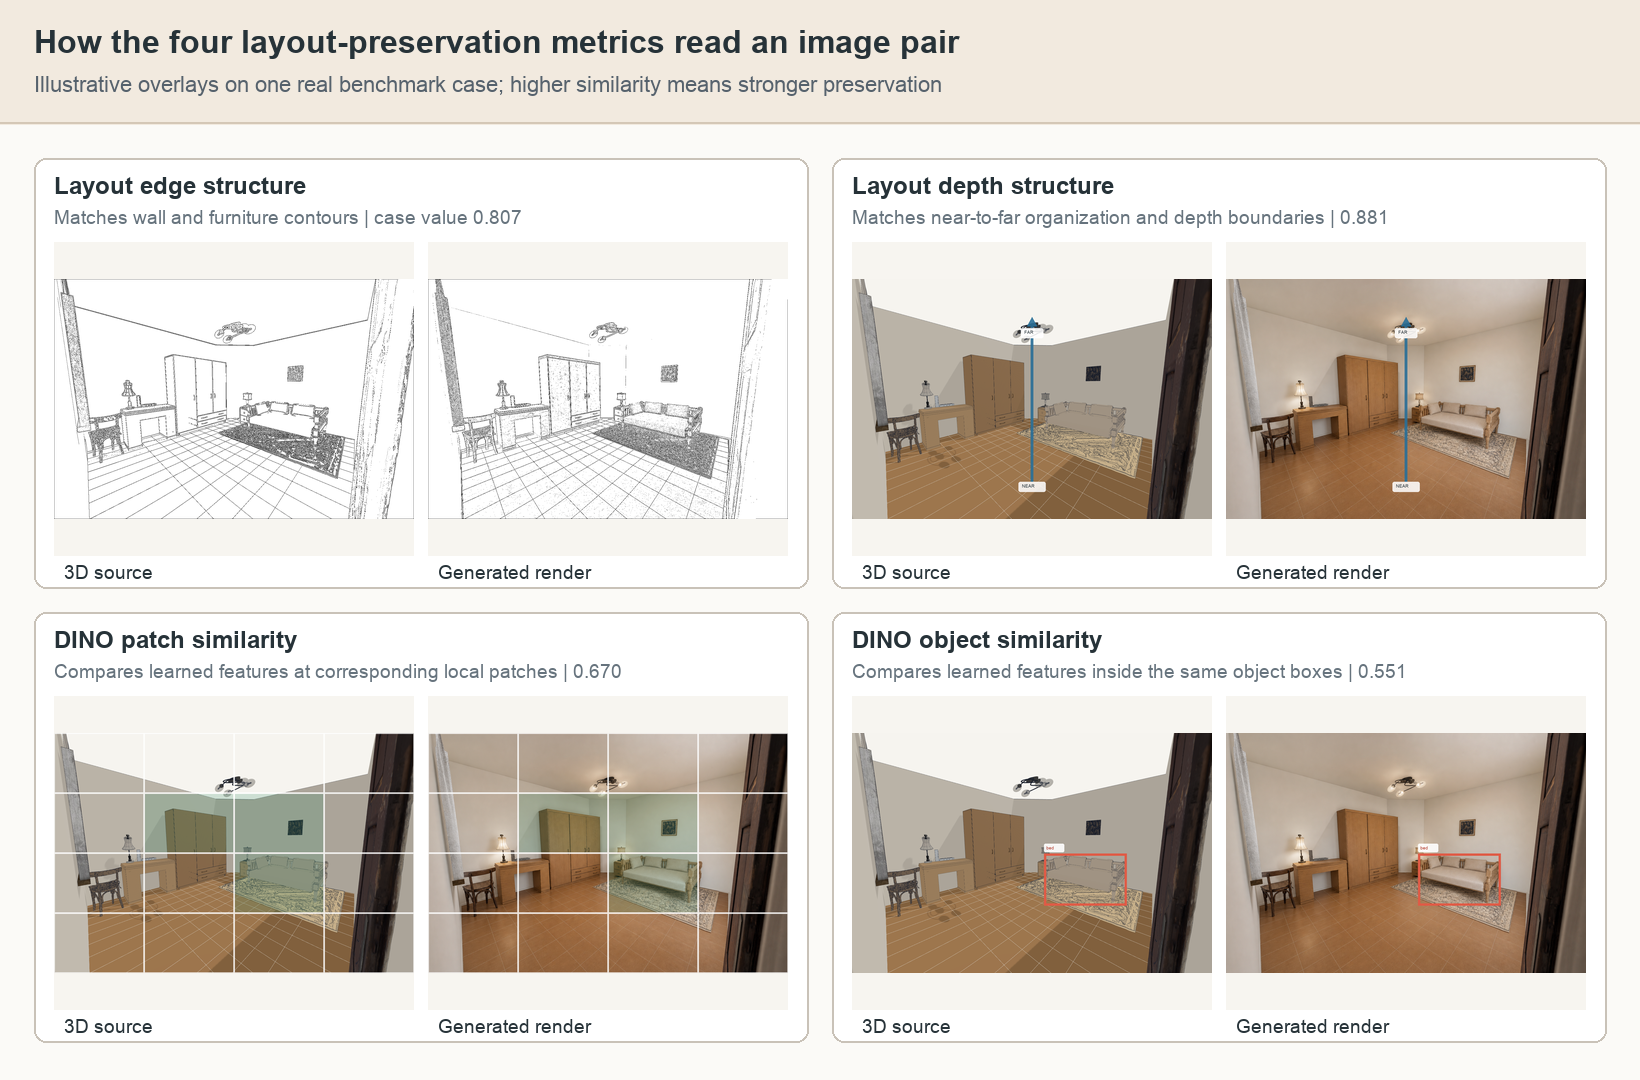
\includegraphics[width=0.96\textwidth]{figures/chapter4/image_flow_cases/image_metric_explanations.png}
\caption{Visual interpretation of the four layout-preservation metrics.}
\label{fig:image-metric-explanations}
\end{figure}

The rendering macro score is the unweighted mean of the four preservation metrics. It summarizes layout preservation across structure, depth, local regions, and visible objects. This score does not directly measure style, lighting, or aesthetic quality. A render may preserve the layout well but still look visually plain, or look attractive while changing the room structure. Therefore, the macro score is interpreted together with preset fidelity, runtime, and qualitative examples in the later experiments.

\subsection{Localized Image Editing Metrics}

The localized image-editing metrics evaluate two aspects: whether the requested edit is successfully applied and whether unrelated parts of the room are preserved. The main metric is the human edit score, based on an operation-specific rubric for add, recolor, remove, and replace requests.

The scoring rules check whether the requested edit is actually applied, whether it affects the correct object or area, whether the camera view and room structure stay the same, whether unrelated objects are kept unchanged, and whether there are no obvious visual errors. Each relevant check is marked as pass or fail, and the final score is the number of passed checks divided by the total number of checks. These annotations are done by a single rater for this thesis, not by multiple raters in a blinded user study.

Automated edge and depth metrics are also used to estimate structural preservation. They are interpreted together with the human edit score because a nearly unchanged image may preserve structure well but fail to perform the requested edit. A successful edited render should therefore satisfy the requested local change while keeping the camera, room shell, openings, and unrelated furniture stable.

\subsection{Preset Fidelity and Operational Cost}

Preset fidelity is a supporting generation metric on a 0--1 scale. It checks whether style, lighting, and scenery intent remain recognizable in the output; 0.75 is used as the operational pass threshold. Runtime and provider token counts are reported separately as efficiency indicators. They are not included in the structural macro score because network latency and workflow-specific provider calls affect them.

\section{Experiment 1: Photorealistic Rendering}\label{subsec:eval-image-generation-results}

Experiment~1 compares six layout-guided rendering variants. All variants start from the same selected layout, camera view, 3D snapshot, and visual preset. They differ in how much layout evidence and preservation guidance are included in the rendering request. The purpose is to test whether stronger layout guidance improves preservation of the selected room structure and furniture arrangement.

The six variants are organized by the amount of layout guidance used before rendering. \textbf{Snapshot Prompt (SP)} uses the source snapshot and a short rendering instruction. \textbf{Visible-Object Contract (CO)} adds visible-object information, making the main objects in the selected camera view explicit. \textbf{Contract with Preservation Constraints (CP)} adds constraints that specify which room elements, openings, and furniture arrangements should remain stable. \textbf{Locked Geometry Reference (LG)} provides an additional geometry reference to strengthen structural guidance. \textbf{Layout-Preservation Check (LVP)} refines the preservation constraints before rendering. \textbf{Snapshot with Edge/Silhouette Guidance (SE-ESG)} is the proposed workflow, where structural boundaries are explicitly marked to guide photorealistic rendering. Figure~\ref{fig:image-create-guidance-inputs} shows the image-based guidance inputs used by these variants, and Figure~\ref{fig:image-create-variant-outputs} shows their outputs for one shared source case.

\begin{figure}[H]
\centering
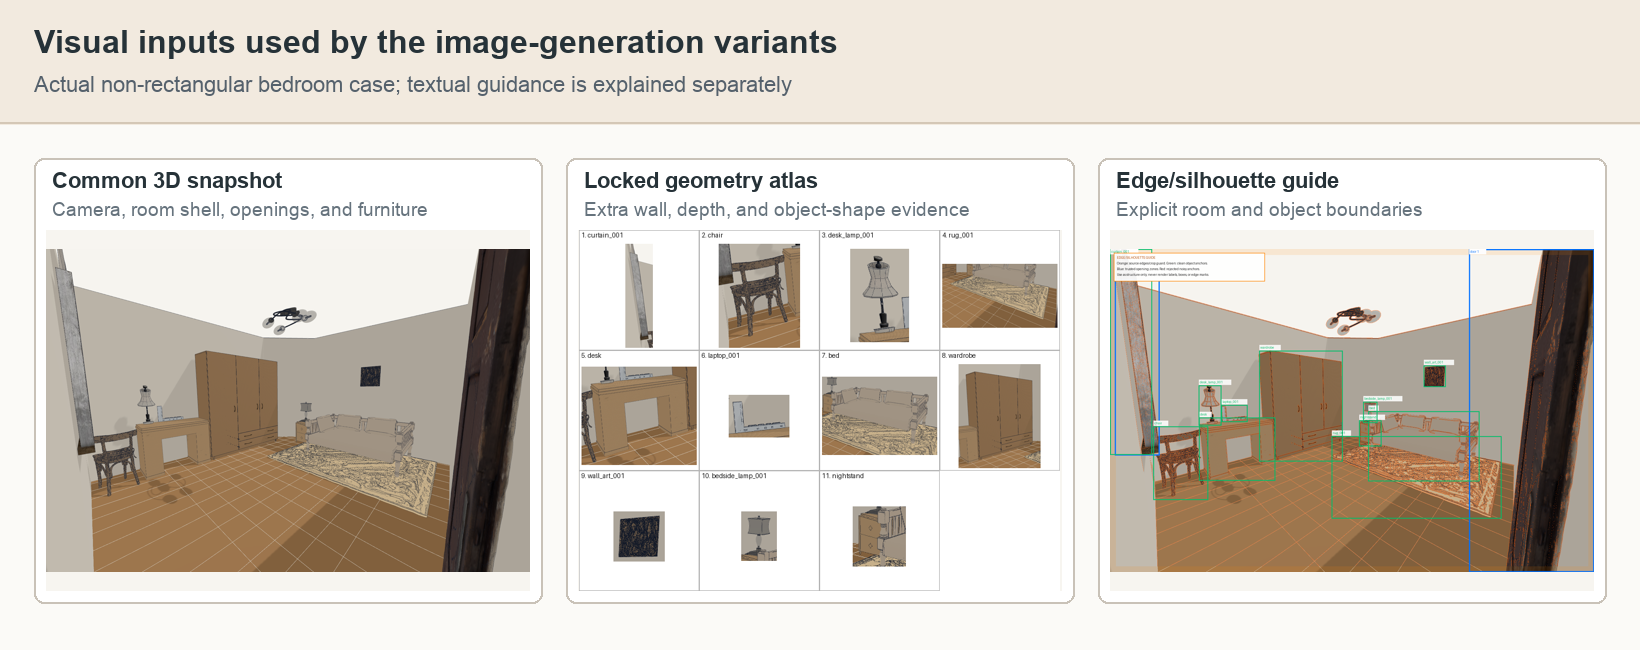
\includegraphics[width=0.96\textwidth]{figures/chapter4/image_flow_cases/create_variant_inputs.png}
\caption{Image-based guidance inputs used by the generation variants.}
\label{fig:image-create-guidance-inputs}
\end{figure}

\begin{figure}[H]
\centering
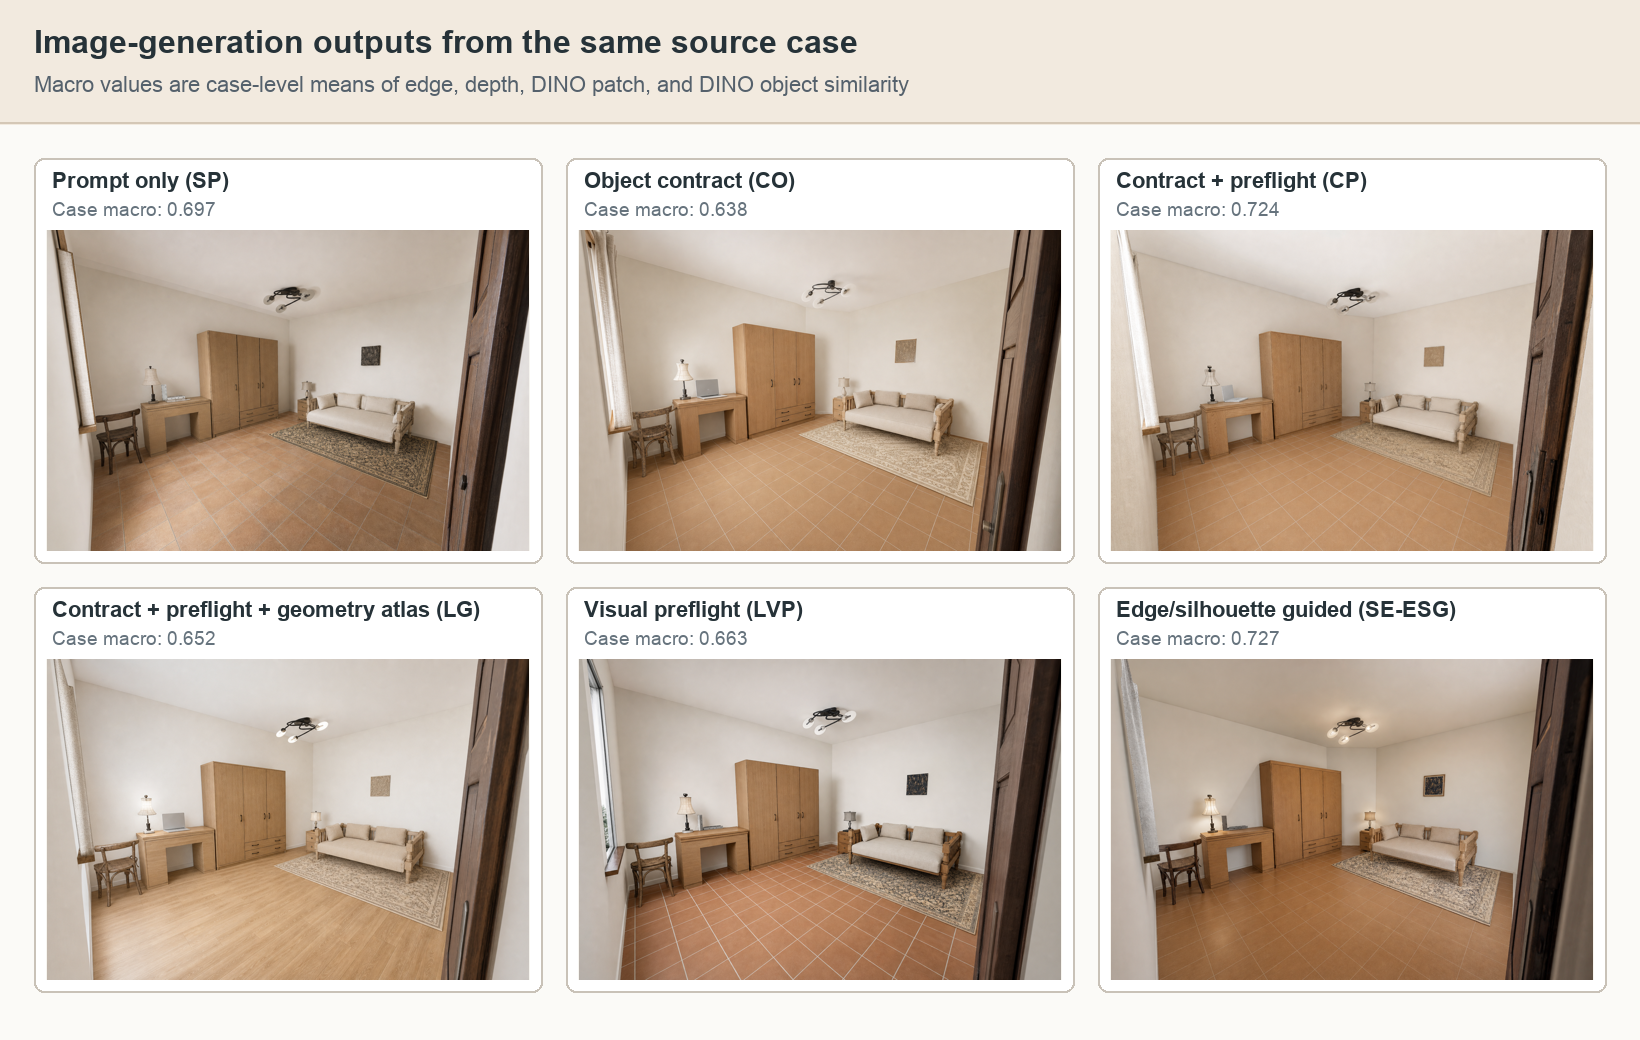
\includegraphics[width=0.96\textwidth]{figures/chapter4/image_flow_cases/create_variant_outputs.png}
\caption{Outputs of the six image-generation variants for one shared source case.}
\label{fig:image-create-variant-outputs}
\end{figure}

Each rendering case is executed twice to capture run-to-run variation from the image model. Table~\ref{tab:8-1} reports the macro layout-preservation results across the two repeated runs.

\begingroup
\small
\setlength{\tabcolsep}{4pt}
\renewcommand{\arraystretch}{1.15}
\begin{xltabular}{\textwidth}{|>{\raggedright\arraybackslash}X|>{\raggedright\arraybackslash}X|>{\raggedright\arraybackslash}X|>{\raggedright\arraybackslash}X|>{\raggedright\arraybackslash}X|>{\raggedright\arraybackslash}X|}
\caption{Macro image-flow results across the two repeated create-flow runs.}\label{tab:8-1}\\
\hline
\textbf{Variant} & \textbf{Macro \(\mu \pm \sigma\)} & \textbf{Edge} & \textbf{Depth} & \textbf{DINO patch} & \textbf{DINO object} \\
\hline
SE-ESG & \textbf{0.587} \(\pm\) 0.112 & \textbf{0.606} & 0.727 & \textbf{0.570} & 0.445 \\
\hline
SP & 0.577 \(\pm\) 0.096 & 0.552 & \textbf{0.731} & 0.555 & \textbf{0.469} \\
\hline
LVP & 0.554 \(\pm\) 0.095 & 0.530 & 0.695 & 0.543 & 0.449 \\
\hline
LG & 0.511 \(\pm\) 0.080 & 0.470 & 0.680 & 0.501 & 0.395 \\
\hline
CP & 0.503 \(\pm\) 0.090 & 0.476 & 0.665 & 0.495 & 0.377 \\
\hline
CO & 0.499 \(\pm\) 0.085 & 0.468 & 0.651 & 0.502 & 0.373 \\
\hline
\end{xltabular}
\endgroup

The results show that Snapshot with Edge/Silhouette Guidance (SE-ESG) achieves the highest macro mean among the tested variants. It reaches 0.587, ahead of Snapshot Prompt (SP) at 0.577 and Layout-Preservation Check (LVP) at 0.554. The improvement mainly comes from edge structure and DINO patch similarity, which are closely related to visible layout preservation. However, SE-ESG does not dominate every individual component: SP remains slightly higher on depth structure and DINO object similarity. The correct conclusion is therefore that SE-ESG provides the best overall preservation trade-off, not that it is best on every metric.

Preset fidelity is used as a supporting check. The evaluator scores whether the generated render follows the requested style, lighting, and scenery preset. A score of 0.75 is used as the operational pass threshold. Figure~\ref{fig:8-5} summarizes the preset-fidelity results after rerunning the complete rendering benchmark. The results show that all rendering variants pass the threshold, with an overall mean of 0.930. SE-ESG reaches 0.918, which is still clearly above the threshold. This means that the main difference between variants should be interpreted mainly through layout preservation, not preset following.

\begin{figure}[H]
\centering
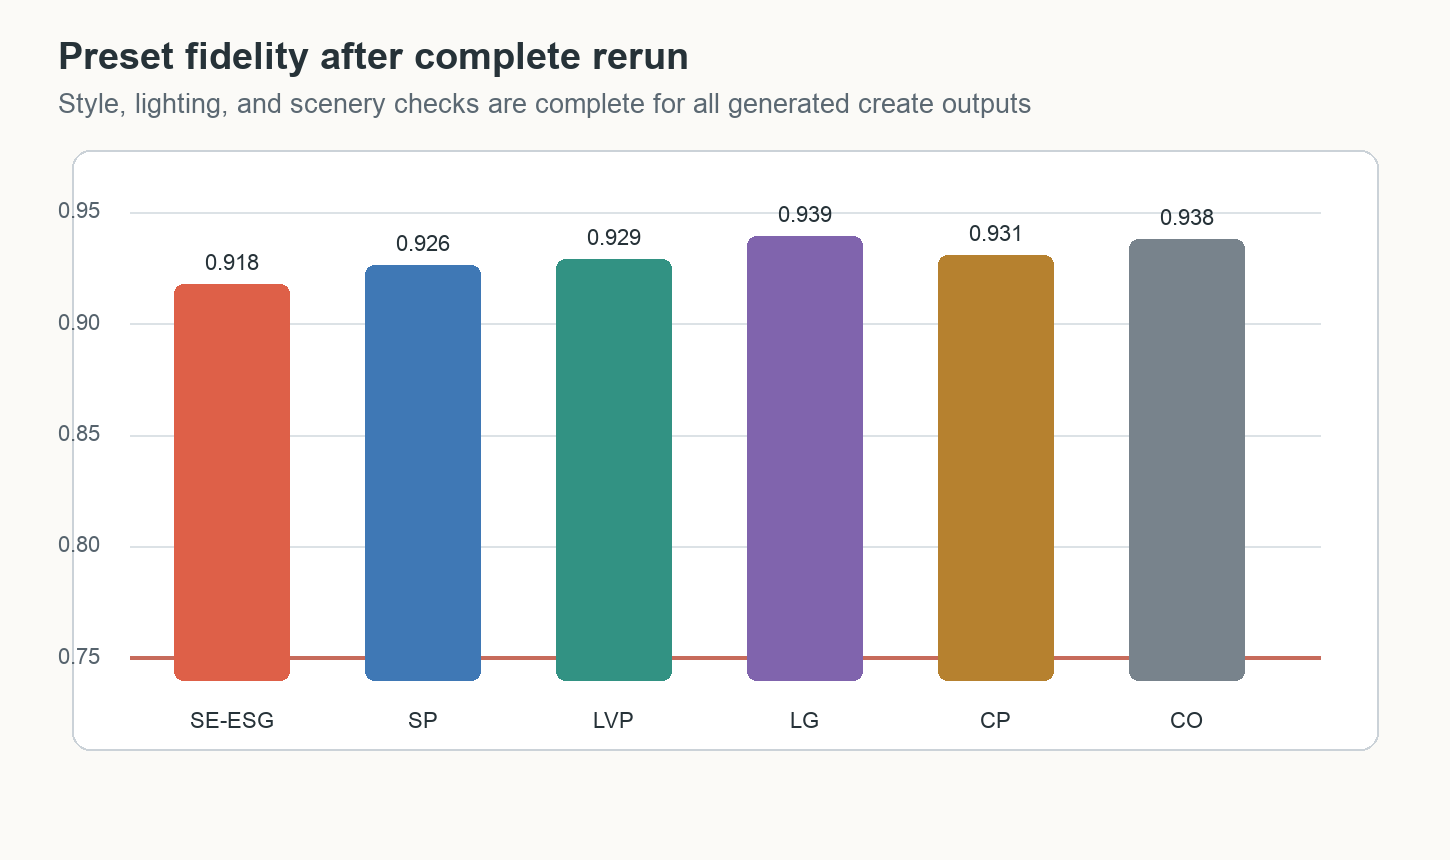
\includegraphics[width=0.92\textwidth]{figures/chapter4/figure_14_preset_fidelity.png}
\caption{Preset-fidelity results after rerunning the complete create benchmark.}
\label{fig:8-5}
\end{figure}

The operational measurements provide deployment context rather than the main quality ranking. Runtime includes network latency, workflow-specific image-model calls, and different reference-image policies. SE-ESG has the lowest observed mean runtime in this implementation, but this should not be interpreted as an inherent property of the method because its request mode and reference package differ from the other variants. Table~\ref{tab:8-2} reports the observed runtime and token logs used for this operational reading.

\begingroup
\small
\setlength{\tabcolsep}{4pt}
\renewcommand{\arraystretch}{1.15}
\begin{xltabular}{\textwidth}{|>{\raggedright\arraybackslash}X|>{\centering\arraybackslash}X|>{\centering\arraybackslash}X|>{\centering\arraybackslash}X|}
\caption{Observed end-to-end runtime and provider-reported token usage for image-flow workflows.}\label{tab:8-2}\\
\hline
\textbf{Variant} & \textbf{Runtime (s)} & \textbf{Input tokens} & \textbf{Output tokens} \\
\hline
SE-ESG & \textbf{55.21} \(\pm\) 2.22 & 4,087 \(\pm\) 56 & \textbf{1,372} \(\pm\) 0 \\
\hline
SP & 73.76 \(\pm\) 7.22 & 6,284 \(\pm\) 0 & \textbf{1,372} \(\pm\) 0 \\
\hline
LVP & 72.13 \(\pm\) 12.96 & 9,646 \(\pm\) 170 & 1,544 \(\pm\) 22 \\
\hline
LG & 75.62 \(\pm\) 3.39 & \textbf{3,230} \(\pm\) 166 & 1,544 \(\pm\) 22 \\
\hline
CP & 69.32 \(\pm\) 6.67 & 11,096 \(\pm\) 305 & 1,544 \(\pm\) 22 \\
\hline
CO & 67.61 \(\pm\) 4.29 & 7,874 \(\pm\) 140 & \textbf{1,372} \(\pm\) 0 \\
\hline
\end{xltabular}
\endgroup

Overall, Experiment~1 supports using Snapshot with Edge/Silhouette Guidance (SE-ESG) as the main rendering workflow. It gives the best macro preservation trade-off while still satisfying the visual preset requirement. The remaining limitation is that layout-guided rendering can still drift at the object level in complex views, especially when the image model changes silhouettes, object details, or local furniture appearance while improving realism.

\section{Experiment 2: Localized Image Editing}\label{subsec:eval-image-editing-results}

Experiment~2 evaluates whether the localized editing workflow improves edit success while preserving unrelated room structure. The experiment compares two variants. The first variant is \textbf{Object-Scope Target Validation (OS)}, which uses the source render, edit instruction, selected target object or marked region, and preservation constraints. The second variant is the \textbf{Prompt-Image-Only Baseline (Prompt)}, which uses the source render and edit instruction without the same explicit target scope and preservation information.

The benchmark contains 32 matched edit requests, executed twice for each variant. The requests are divided into four operation types: add, recolor, remove, and replace. Figure~\ref{fig:image-edit-variant-comparison} shows one matched recolor example, where the two variants are applied to the same source render and edit instruction. This example illustrates the main purpose of object-scope editing: the target object should change, while the room shell, camera view, openings, and unrelated furniture should remain stable.

\begin{figure}[H]
\centering
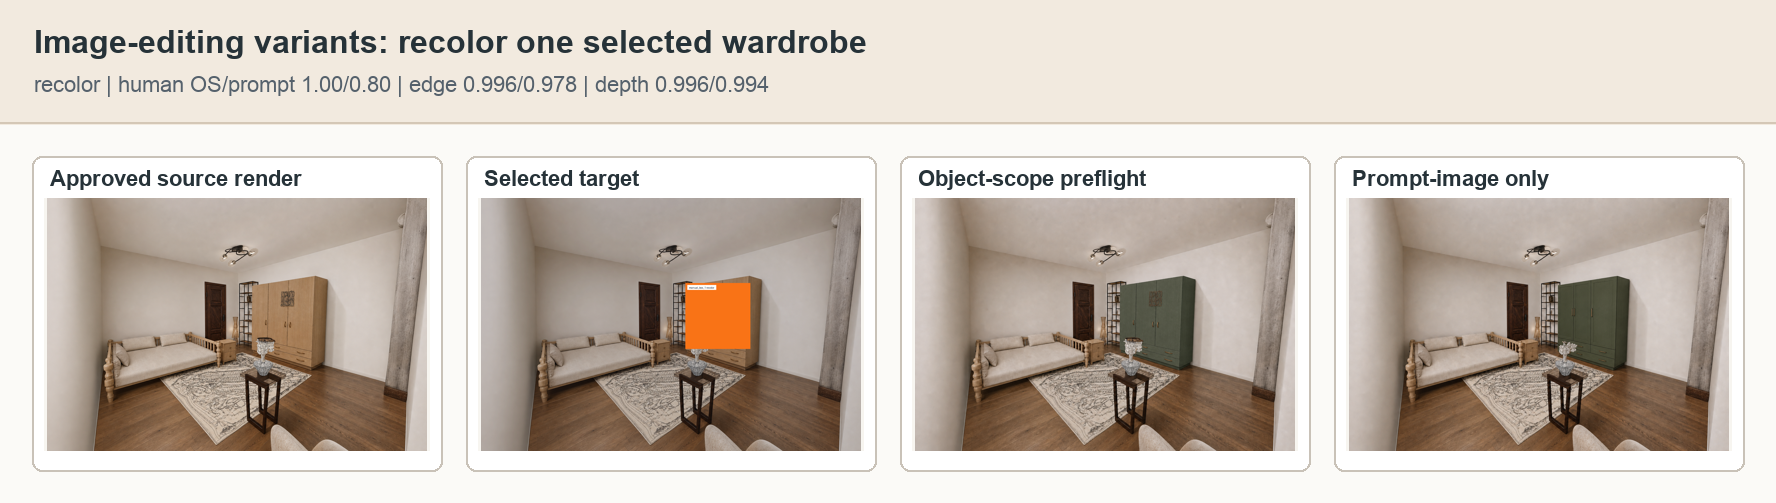
\includegraphics[width=0.96\textwidth]{figures/chapter4/image_flow_cases/edit_variant_comparison.png}
\caption{The two image-editing variants on one matched recolor request.}
\label{fig:image-edit-variant-comparison}
\end{figure}

Table~\ref{tab:8-3} summarizes the manual edit scores by operation.

\Needspace{18\baselineskip}
\begin{table}[!htbp]
\centering
\small
\setlength{\tabcolsep}{4pt}
\renewcommand{\arraystretch}{1.15}
\caption{Image-editing manual score and paired metric deltas by operation.}\label{tab:8-3}
\begin{tabularx}{\textwidth}{|>{\raggedright\arraybackslash}p{1.8cm}|>{\centering\arraybackslash}p{1.2cm}|>{\raggedright\arraybackslash}p{3.2cm}|>{\raggedright\arraybackslash}X|}
\hline
\textbf{Operation} & \textbf{n pairs} & \textbf{Manual score OS / Prompt} & \textbf{Main reading} \\
\hline
Overall & 64 & \textbf{0.956} / 0.897 & Object-scope preflight improves semantic edit success; prompt-only stays closer to source structure. \\
\hline
Add & 16 & 0.963 / \textbf{0.975} & Both variants usually succeed; the difference is not significant. \\
\hline
Recolor & 16 & \textbf{1.000} / 0.775 & Object-scope preflight is clearly better because the target object and color are explicit. \\
\hline
Remove & 16 & \textbf{0.975} / 0.963 & The two variants are close, with a small object-scope advantage. \\
\hline
Replace & 16 & \textbf{0.887} / 0.875 & Replacement is the hardest operation for both variants. \\
\hline
\end{tabularx}
\end{table}

Overall, Object-Scope Target Validation achieves a higher manual edit score than the Prompt-Image-Only Baseline, with 0.956 compared with 0.897. The largest improvement appears in recolor requests, where OS reaches 1.000 while Prompt reaches 0.775. This result shows that explicit target scope is especially useful when the edit must affect one visible object without changing the rest of the room.

For add and remove operations, both variants perform well. Prompt is slightly higher on add, while OS is slightly higher on remove. Replacement is the hardest operation for both variants, with OS at 0.887 and Prompt at 0.875. These results suggest that replacement requires more precise control because the model must change object identity while preserving location, scale, and surrounding furniture.

The structural preservation metrics are interpreted together with the manual edit score. A prompt-image-only result may sometimes stay closer to the source image because it changes less, but this can also indicate under-editing when the requested operation is not fully performed. For this reason, the main conclusion of Experiment~2 is that object-scope target validation improves semantic edit success, especially for targeted recolor edits, while still keeping the surrounding room structure reasonably stable.

\section{Discussion}\label{subsec:eval-image-discussion}

The image evaluation supports three conclusions. First, snapshot-guided rendering is better treated as a structured workflow than as a plain text prompt. SE-ESG gives the best macro trade-off among the tested create variants. Second, preset fidelity is sufficiently high in the completed checks to support using style, lighting, and scenery presets as controllable user-facing options. Third, object-scope preflight improves localized edit success, especially for recolor, although it costs more tokens and can reduce edge/depth similarity when the edit is more decisive.

\section{Threats to Validity}\label{sec:eval-threats-to-validity}

\noindent\textbf{Internal validity.}
Provider-side model updates, network conditions, and stochastic generation may influence both output quality and runtime. Matched source cases, fixed variant definitions, and two repeated runs reduce confounding, but they do not remove provider variability. The operational-cost comparison is additionally affected by differences in provider endpoint, reference-image count, and workflow call graph. Provider token accounting may also differ across generation, editing, and multi-image requests. The reported values are therefore descriptive workflow logs rather than normalized estimates of computational efficiency.

\noindent\textbf{External validity.}
The generation benchmark contains 14 selected bedroom and living-room layouts, while the editing benchmark contains 32 operation-specific requests. These cases cover several geometries and edit types, but they do not represent all room types, camera views, visual styles, or user instructions.

\noindent\textbf{Construct validity.}
Edge, depth, and DINO similarities capture complementary aspects of structural preservation, but they cannot fully measure realism or design quality. Preset fidelity is vision-model-assisted, and the human edit scores are single-rater thesis annotations rather than a blinded multi-rater user study.

\noindent\textbf{Conclusion validity.}
The number of cases and two repeated runs limit statistical power. Confidence intervals and Holm adjustment reduce overstatement, but the findings remain evidence for the tested workflows and provider setting rather than proof that the same ranking will hold for every future model version.
